\documentclass[11pt,letterpaper]{article}
\usepackage[margin=1in,headheight=14pt]{geometry}
\usepackage[T1]{fontenc}
\usepackage{newtxtext,newtxmath}
\usepackage{amsmath,booktabs,tabularx,array,graphicx,xcolor,enumitem,microtype,fancyhdr,titlesec,xurl}
\usepackage{float}
\usepackage[colorlinks=true,urlcolor=blue,linkcolor=black]{hyperref}
\setlength{\parindent}{0pt}
\setlength{\parskip}{4pt}
\setlength{\emergencystretch}{1em}
\setlength{\abovedisplayskip}{4pt}
\setlength{\belowdisplayskip}{4pt}
\setlength{\textfloatsep}{10pt}
\setlength{\floatsep}{8pt}
\setlength{\intextsep}{8pt}
\renewcommand{\arraystretch}{1.1}
\titleformat{\section}{\normalsize\bfseries}{\thesection.}{.5em}{}
\titleformat{\subsection}{\normalsize\bfseries}{\thesubsection}{.5em}{}
\titlespacing*{\section}{0pt}{8pt}{4pt}
\titlespacing*{\subsection}{0pt}{6pt}{3pt}
\setlist[itemize]{leftmargin=*,nosep}
\pagestyle{fancy}\fancyhf{}
\fancyhead[L]{\footnotesize IEOR E4004: Optimization Models and Methods}
\fancyhead[R]{\footnotesize Group 21L | Milestone 5}
\fancyfoot[C]{\thepage}
\renewcommand{\headrulewidth}{.3pt}
\graphicspath{{figures/}}
\urlstyle{same}
\raggedbottom


\begin{document}
{\large\bfseries Fresh Product Assortment and Stocking Allocation\\
Across Three Dingdong Fulfillment Stores\par}
\textbf{Milestone 5: Results and Sensitivity Analysis}\\
Group 21L \hfill November 18, 2026\\
Jiayue Zhang, Yue Peng, Andrew Bian, Langzhuo Liu, and Hang Seo Cho

\section{Problem and managerial decision}
A regional fulfillment planner chooses which of 29 candidate products
each of three Dingdong stores may carry and how much new stock to
deliver daily over June 26--July 2, 2024. Decisions use information
available through June 25. Limited assortment space, storage, supply,
and a short assumed shelf life require trade-offs between service and
inventory exposure. We jointly optimize selection and deliveries,
then examine resource sensitivity and performance on common evaluation
demand paths. The results support targeted assortment and storage pilots, while common-path evaluation identifies limits of the fixed-delivery policy.

\section{Data and demand construction}\label{sec:data}
FreshRetailNet-50K provides normalized sales and hourly stockout information
(Dingdong-Inc., 2025). The sample comprises anonymous city 0, stores 18,
145, and 235, and 29 common products in second-category codes 25 and 28.
The 90-day training period, March 28--June 25, contains 7,830 daily records.
Recovery estimates lost demand from comparable in-stock hours while
preserving observed sales, addressing censored demand
(Shi et al., 2016). Hierarchical matches use store, product, hour,
day type and activity, relaxing activity and day-type matching when necessary.

\begin{table}[H]\centering
\caption{Historical means and supplied point forecasts, in normalized units.}
\begin{tabular}{lrrr}\toprule
Store & Daily sales & Daily recovered demand & Seven-day forecast\\\midrule
18 & 44.88 & 53.35 & 408.33\\
145 & 39.31 & 47.04 & 378.05\\
235 & 39.31 & 47.08 & 348.48\\\bottomrule
\end{tabular}\end{table}

Let $\mu_{sp}$ be mean recovered demand over June 19--25 and
$g_{s,w(t)}$ the store weekday factor estimated over May 29--June 25.
The point forecast is $\bar d_{spt}=\mu_{sp}g_{s,w(t)}$, and original
scenario demand is $d_{spt\omega}=\kappa_\omega\bar d_{spt}$.
The factor is the store's weekday-specific mean demand divided by its
overall daily mean. The original low, typical, and high multipliers are
0.942545, 1.045028, and 1.175382, with assumed probabilities 0.3, 0.4, and 0.3.
The optimizer uses the full-precision CSV values. There are 609 forecasts
and 1,827 scenario-demand entries. Each original scenario scales all
stores, products, and days together.



\paragraph{Holdout preparation and validation.}
The holdout contains 609 store-product-day records for June 26--July 2.
The demand team applies training-period Day Type Matching ($k=15$), using only
in-stock March 28--June 25 observations as historical references. Daily checks
confirm complete records, unique keys, and recovered demand at least as large
as observed sales. The columns \texttt{sale\_amount} and \texttt{demand} retain
observed sales and estimated recovered demand, respectively.

\clearpage
\section{Complete optimization model}
\subsection{Sets, parameters, and assumptions}
Let $S=\{18,145,235\}$ index stores, $P$ index 29 products,
$T=\{1,\ldots,7\}$ index planning days, and
$\Omega=\{\mathrm{low},\mathrm{typical},\mathrm{high}\}$ index complete
demand scenarios. Inputs are demand $d_{spt\omega}$ and probabilities
$\pi_\omega\geq0$, with $\sum_\omega\pi_\omega=1$.

\begin{table}[H]\centering
\caption{Resource parameters and relative loss weights.}
\begin{tabularx}{\linewidth}{lXl}\toprule
Symbol & Meaning and source & Base value\\\midrule
$C_{st}$ & Pre-sale inventory capacity, training daily-sales P90 proxy
& 51.25, 46.93, 46.41\\
$R_t$ & Shared daily new supply, regional daily-sales P90 proxy & 144.43\\
$K_s$ & Assumed weekly assortment upper limit & 20\\
$\alpha,\beta$ & Assumed penalties per unit of shortage and expiration & 5, 1\\
$h,\tau$ & Assumed penalties per unit of overnight and terminal stock & 0.2, 0.5\\
$Q_{spt}$ & Derived delivery bound & $\min\{C_{st},R_t\}$\\
$B_{spt\omega}$ & Derived minimum-linearization bound & $\max\{C_{st},d_{spt\omega}\}$\\\bottomrule
\end{tabularx}\end{table}

Weekly assortment and all daily deliveries are determined at the June 25
cutoff. A single delivery arrives before daily sales. Initial old stock
is zero. All products are assumed sellable on arrival day and the next
day, following a two-period inventory structure (Chen \& Sapra, 2013).
New stock left at day-end becomes old stock the next morning. Unsold
old stock expires at day-end. FIFO is imposed. Demand is exogenous,
with no substitution, transfer, or backordering. Demand for excluded
products counts as unmet. Category codes impose no assortment-coverage
constraint. Quantities and capacity proxies share the normalized scale.

\subsection{Variables}
All scenario-indexed stock and sales variables are constrained outcomes
of the shared selection and delivery decisions. Lower-case report
symbols follow the TA's consistency feedback. Code correspondence is
included to preserve traceability.
\begin{table}[H]\centering
\begin{tabularx}{\linewidth}{llX}\toprule
Symbol & Code & Meaning and domain\\\midrule
$z_{sp}$ & \texttt{z} & Binary product permission for the week\\
$q_{spt}$ & \texttt{q} & Nonnegative new delivery\\
$o_{spt\omega}$ & \texttt{O} & Nonnegative start-of-day old stock\\
$v_{spt\omega}$ & \texttt{V} & Nonnegative pre-sale inventory\\
$a_{spt\omega}$ & \texttt{A} & Nonnegative total sales\\
$a^o_{spt\omega},a^n_{spt\omega}$ & \texttt{Sold}, \texttt{Snew} & Nonnegative old- and new-stock sales\\
$\ell_{spt\omega}$ & \texttt{L} & Nonnegative new stock remaining at day-end\\
$w_{spt\omega}$ & \texttt{W} & Nonnegative expired old stock\\
$u_{spt\omega}$ & \texttt{U} & Nonnegative unmet demand\\
$b^a_{spt\omega},b^o_{spt\omega}$ & \texttt{bA}, \texttt{bO} & Binary minimum-branch indicators\\\bottomrule
\end{tabularx}\end{table}
All non-binary quantities are continuous normalized units.

\subsection{Objective}
\begin{equation}
\begin{aligned}
\min J&=\sum_{\omega\in\Omega}\pi_\omega J_\omega,\\
J_\omega&=\sum_{s,p,t}(\alpha u_{spt\omega}+\beta w_{spt\omega})
+h\sum_{s,p}\sum_{t=1}^{6}\ell_{spt\omega}
+\tau\sum_{s,p}\ell_{sp7\omega}.
\end{aligned}
\end{equation}
The planner minimizes relative loss from shortages, expiration,
overnight carryover, and terminal new inventory. Day-7 new stock receives
the terminal charge. Earlier new-stock balances receive the overnight
charge. These coefficients express relative preferences.

\subsection{Constraints}
All expressions apply to relevant stores, products, days, and scenarios
unless otherwise specified.
\begin{equation}
\sum_p z_{sp}\leq K_s,\qquad 0\leq q_{spt}\leq Q_{spt}z_{sp}.
\end{equation}
Each store permits at most $K_s$ products and deliveries require selection.
Permission alone allows a zero delivery.
\begin{equation}
o_{sp1\omega}=0,\qquad o_{spt\omega}=\ell_{sp,t-1,\omega}\quad(t=2,\ldots,7).
\end{equation}
Old stock starts at zero. Yesterday's remaining new stock becomes old stock.
\begin{equation}v_{spt\omega}=o_{spt\omega}+q_{spt}.\end{equation}
Pre-sale stock combines carryover and today's new deliveries.
\begin{equation}\sum_p v_{spt\omega}\leq C_{st}\quad(\forall s,t,\omega).\end{equation}
The same delivery plan must fit storage under every planning scenario.
\begin{equation}\sum_s\sum_p q_{spt}\leq R_t\quad(\forall t).\end{equation}
All three stores share the regional daily new-supply allowance.
\begin{equation}
\begin{aligned}
a_{spt\omega}&\leq v_{spt\omega},&a_{spt\omega}&\leq d_{spt\omega},\\
a_{spt\omega}&\geq v_{spt\omega}-B_{spt\omega}b^a_{spt\omega},&
a_{spt\omega}&\geq d_{spt\omega}-B_{spt\omega}(1-b^a_{spt\omega}).
\end{aligned}
\end{equation}
These inequalities impose total sales equal to
$\min\{v_{spt\omega},d_{spt\omega}\}$.
\begin{equation}
\begin{aligned}
a^o_{spt\omega}&\leq o_{spt\omega},&a^o_{spt\omega}&\leq d_{spt\omega},\\
a^o_{spt\omega}&\geq o_{spt\omega}-B_{spt\omega}b^o_{spt\omega},&
a^o_{spt\omega}&\geq d_{spt\omega}-B_{spt\omega}(1-b^o_{spt\omega}).
\end{aligned}
\end{equation}
Old-stock sales equal $\min\{o_{spt\omega},d_{spt\omega}\}$, enforcing FIFO.
\begin{equation}
a^n_{spt\omega}=a_{spt\omega}-a^o_{spt\omega},\qquad
\ell_{spt\omega}=q_{spt}-a^n_{spt\omega}.
\end{equation}
New stock meets the remaining demand. Its unsold balance carries over once.
\begin{equation}
w_{spt\omega}=o_{spt\omega}-a^o_{spt\omega},\qquad
u_{spt\omega}=d_{spt\omega}-a_{spt\omega}.
\end{equation}
Unsold old stock expires. All unserved demand is recorded as shortage.
\begin{equation}
\begin{aligned}
&z_{sp},b^a_{spt\omega},b^o_{spt\omega}\in\{0,1\},\\
&q_{spt},o_{spt\omega},v_{spt\omega},a_{spt\omega},a^o_{spt\omega},
a^n_{spt\omega},\ell_{spt\omega},w_{spt\omega},u_{spt\omega}\geq0.
\end{aligned}
\end{equation}
Selection and branch indicators are binary. Inventory flows are nonnegative.
Capacity bounds both $v$ and $o$ by $C_{st}$, validating the stated
linearization bounds.

\clearpage

\section{Optimization decisions and initial results}
The original M4 plan permits 20 products per store and delivers 958.11 normalized
units over seven days. Store totals are 343.31, 316.83, and 297.97 for stores 18,
145, and 235. These are concrete weekly selection and daily delivery decisions.

\subsection{Solution status and verification}
Gurobi 13.0.3 solves the 18,966-variable, 26,260-constraint model with a
300-second limit, requested gap of 0.1\%, seed 21, and four threads.
The incumbent loss is 1,229.3058, with lower bound 1,212.6949 and achieved gap
1.3512\%. A separate FIFO simulation reconstructs the solution and objective.
Maximum constraint and inventory discrepancies are approximately
$3.4\times10^{-13}$. Reported losses use relative penalty points.

\begin{table}[H]\centering
\caption{Original M4 plan on its planning scenarios. Quantities are normalized.}
\begin{tabular}{lrrrrr}\toprule
Scenario & Demand & Sales & Fill rate & Unmet & Expired\\\midrule
Low & 1,069.65 & 939.62 & 87.84\% & 130.03 & 9.33\\
Typical & 1,185.95 & 956.35 & 80.64\% & 229.60 & 1.76\\
High & 1,333.89 & 958.11 & 71.83\% & 375.77 & 0.00\\\bottomrule
\end{tabular}\end{table}

\subsection{Shortage composition identifies different interventions}
In the low scenario, excluded products account for 119.54 of 130.03 unmet units,
approximately 92\%. In the high scenario, selected products with insufficient
stock account for 226.70 of 375.77 unmet units, approximately 60\%.
Assortment expansion and inventory resources therefore address different parts
of the service shortfall (Figure~\ref{fig:shortage}).
\begin{figure}[H]\centering
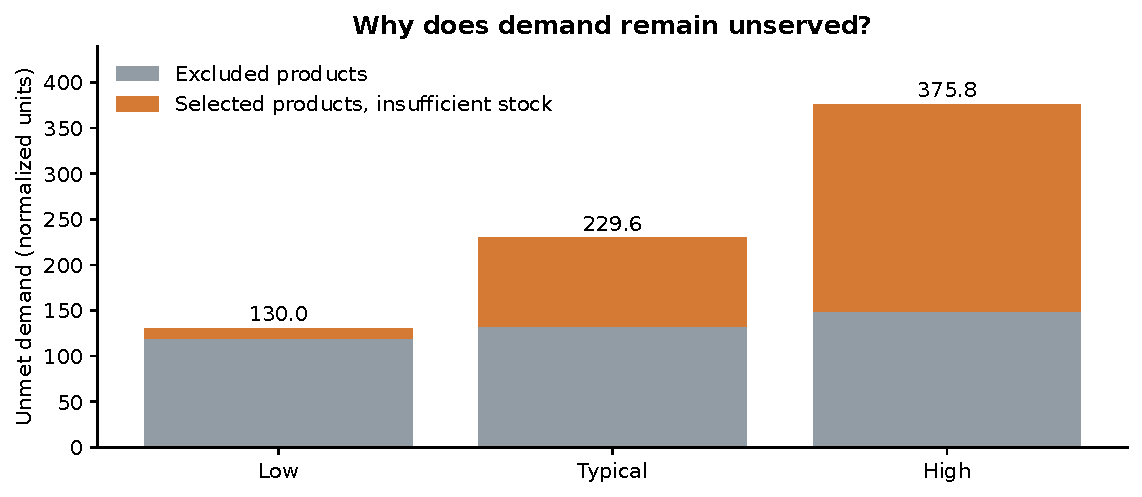
\includegraphics[width=.74\linewidth]{figures/fig01_shortage_sources.pdf}
\caption{Unmet demand from excluded and selected products. All candidate-product
demand remains in the service denominator.}\label{fig:shortage}
\end{figure}

\subsection{Carryover limits usable space}
Storage is binding on 12 of 21 low-scenario store-days in the original plan,
while regional supply has positive slack every day. Carryover occupies storage
before a new delivery arrives. These observations motivate separate experiments
on assortment, storage, and supply. They also motivate the later diagnostic of
fixed deliveries under product-level uncertainty.

\clearpage
\section{Sensitivity analysis and managerial choices}
\subsection{Design, metrics, and numerical precision}
We conduct 14 cases including one base case. Each changes one parameter:
$K=15,20,25,29$; storage and supply factors $0.85,1.00,1.20$ separately;
$\alpha=2,5,10$; $h=0,0.2,0.5$; and $\tau=0.25,0.5,1$, with $\beta=1$.
Cases use a repaired base-plan warm start, a 60-second limit, and the same seed,
thread count, and requested gap as M4. Achieved gaps range from 0.003\% to 3.80\%.
The sensitivity base is a separate incumbent with loss 1,229.2876 and gap 2.16\%.

Sensitivity service is $F=\mathbb{E}[\mathrm{sales}]/\mathbb{E}[\mathrm{demand}]$,
following the code. All cases use the original three planning scenarios.
Expected quantities use their probabilities. Changed-weight plans are also
scored using common base weights $(5,1,0.2,0.5)$.
\begin{table}[H]\centering
\caption{One-parameter resource experiments, with base-weight loss.}
\begin{tabular}{lrrrr}\toprule
Setting & $F$ & Loss & Expired & MIP gap\\\midrule
Base & 79.62\% & 1,229.29 & 3.46 & 2.16\%\\
$K=15$ & 72.99\% & 1,640.44 & 7.66 & 3.80\%\\
$K=25$ & 83.01\% & 1,019.55 & 1.34 & 0.67\%\\
$K=29$ & 83.89\% & 964.86 & 0.86 & 0.32\%\\
Storage $\times0.85$ & 71.62\% & 1,696.98 & 0.20 & 0.10\%\\
Storage $\times1.20$ & 82.49\% & 1,076.74 & 8.64 & 3.22\%\\
Supply $\times0.85$ & 71.89\% & 1,680.47 & 0.00 & 0.003\%\\
Supply $\times1.20$ & 79.62\% & 1,229.27 & 3.43 & 1.97\%\\\bottomrule
\end{tabular}\end{table}

\subsection{What if a store could carry five more products?}
Raising $K$ from 20 to 25 improves service by 3.38 percentage points and lowers
incumbent loss by 17.1\%. Increasing $K$ from 25 to 29 adds 0.89 service points.
Expected excluded-product demand falls from 133.60 to 46.93 and then zero.
Shortages on selected products rise as additional items compete for resources,
while total shortages fall from 243.58 to 203.14 and 192.54 units.
\begin{figure}[H]\centering
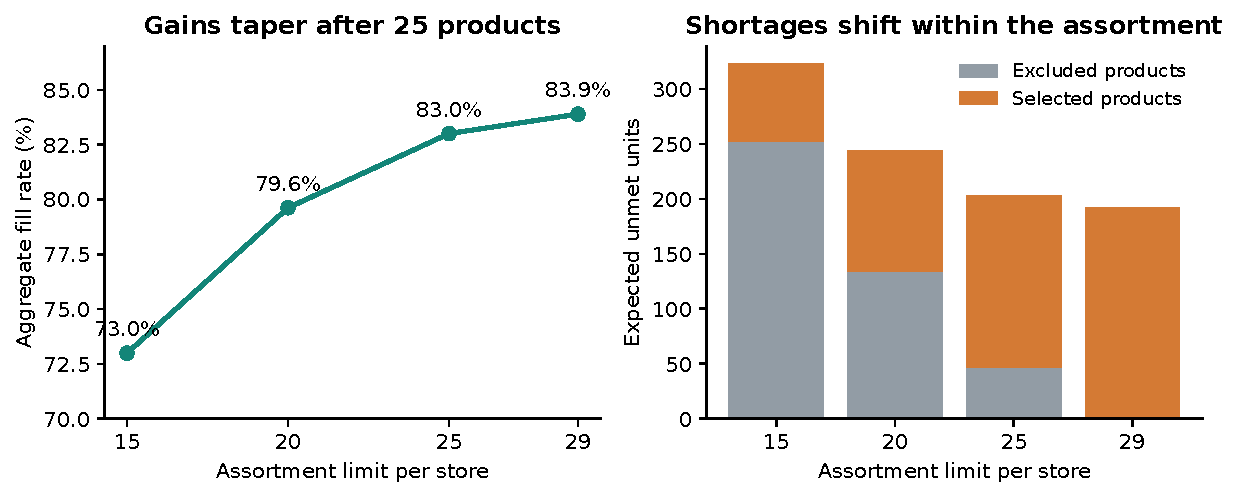
\includegraphics[width=.84\linewidth]{figures/fig03_assortment.pdf}
\caption{Assortment breadth, aggregate service, and shortage composition.}
\label{fig:assortment}
\end{figure}

\clearpage
\subsection{What if storage or supply changes?}
Storage expansion by 20\% raises service by 2.87 points and lowers loss by 12.4\%.
Supply then becomes approximately binding on six of seven days. Supply expansion
alone gives negligible change among the obtained incumbents. Reducing storage
by 15\% costs 8.00 service points, and reducing supply by 15\% costs 7.74 points.
Protecting current supply reliability and purchasing more supply therefore have
different effects in these experiments.
\begin{figure}[H]\centering
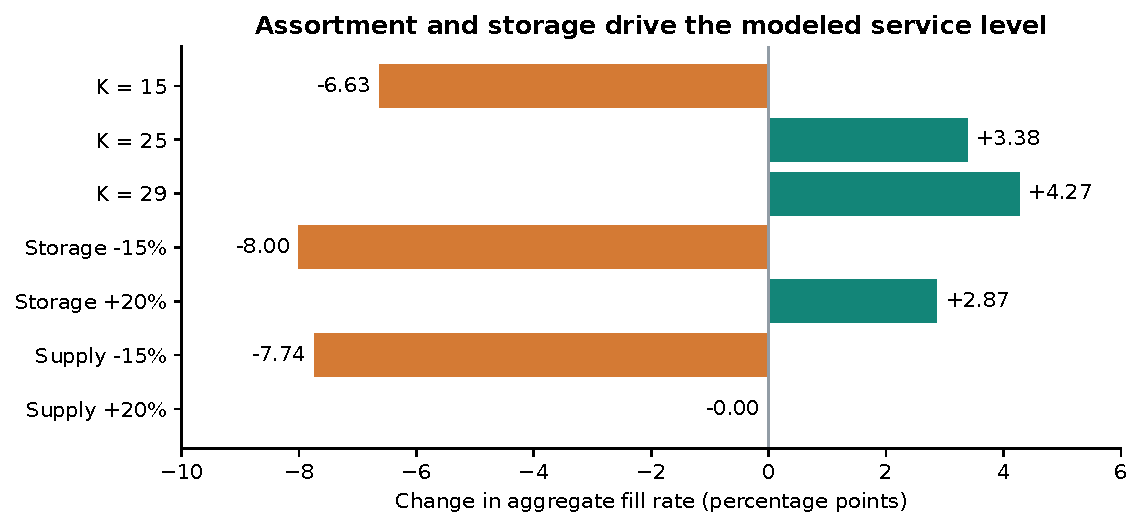
\includegraphics[width=.95\linewidth]{figures/fig04_resource_effects.pdf}
\caption{Service changes from the sensitivity base, in percentage points.
Each bar changes one resource parameter.}\label{fig:resourceeffects}
\end{figure}
Storage expansion increases expected carryover from 32.65 to 83.12 and expiration
from 3.46 to 8.64 units. A storage pilot should measure expiry and turnover along
with service. Actual investment decisions require measured space and cost data,
since our capacities are historical-sales proxies.

\subsection{What if the manager changes the penalty priorities?}
Across the six non-base weight settings, the assortment is unchanged, service
moves by less than 0.03 points, and common-weight loss changes by less than 0.1\%.
For example, $\alpha=2$ and $\alpha=10$ give common-weight losses 1,229.58 and
1,229.29. Expiration changes from 2.36 to 3.50 units. Resource assumptions deserve
priority for validation within the tested ranges.

\subsection{Interpretation using optimization bounds and local duals}
The $K=25$ incumbent loss, 1,019.55, and storage-expansion loss, 1,076.74, are
both below the base lower bound, 1,202.71. Thus the improved resource settings
permit better objective values even accounting for incomplete solution of the
base model. Exact percentage improvements remain incumbent-based.
Supply-expansion and base bounds overlap, qualifying a claim of zero optimal gain.

The supplementary LP analysis fixes all binary variables, including minimum-branch
indicators. Its duals describe local marginal changes within that fixed structure.
They support investigating store space, but their range of validity excludes
integer switching. One-parameter experiments establish separate effects.
Quantifying a joint $K$--storage investment requires a further joint experiment.
Residual MIP gaps qualify interpretations of small decision differences.

\clearpage
\section{Demand uncertainty and Monte Carlo simulation}\label{sec:mc}
\subsection{Cutoff-specific calibration}
We simulate 2,000 complete seven-day demand paths, each containing 609 values,
using seed 21. Forecast errors are calibrated from eight weekly origins,
April 30--June 18. Each forecast uses a recovery file built through its own origin.
Realized targets use full-period recovered demand, so target estimation remains
an uncertainty source. This replaces the earlier six-origin look-ahead version.

The realized-to-forecast ratio is decomposed into store-week, store-day, and
product-day components. Weekly log ratios combine a shared week effect
($\sigma_f=0.055$), store deviation ($\sigma_e=0.051$), and mean log effect
$\mu=0.018$, with estimation error 0.022. Daily and product-level ratios are
resampled within store and store-product pools, rescaled to mean one.
Product-day draws are conditionally independent given their shared factors.

\begin{figure}[H]\centering
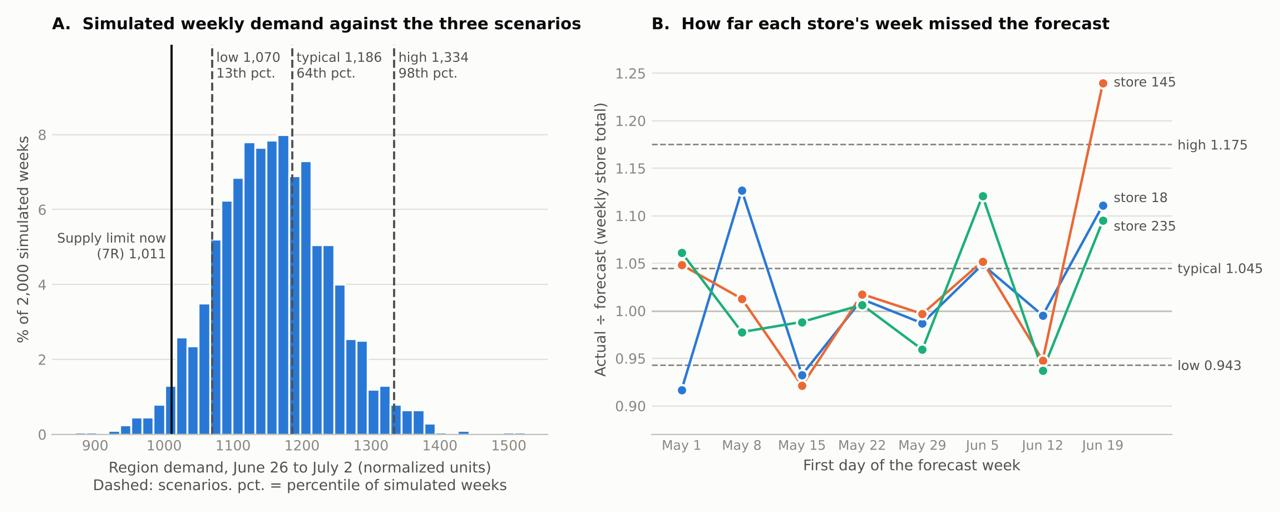
\includegraphics[width=\linewidth]{figures/mc_figure.jpeg}
\caption{Corrected simulation distribution and cutoff-based weekly forecast
errors, supplied by the demand team. The supply line is seven times the daily limit.}
\label{fig:mc}
\end{figure}

\subsection{Distribution and validation}
Regional weekly demand has mean 1,159, median 1,157, and P10--P90 range
1,058--1,263. The corresponding multiplier quantiles are 0.933, 1.020, and 1.113.
The original low, typical, and high scenarios fall near simulated percentiles
13, 64, and 98, respectively. Original high demand is a demanding stress case.
Product-day demand has a much wider central 90\% ratio range, 0.40--1.74.

Leave-one-week-out refitting covers 7 of 8 regional and 22 of 24 store-week totals
within central 80\% intervals. The held-out evaluation week totals 1,106.75,
at approximately the simulation's 27th percentile. Its product-day coverage is
79.1\% for central 80\% intervals. A Saturday demand miss remains visible.
These small-sample checks support the simulated range while retaining
uncertainty about calibration, promotions, and recovery error.

Weekly demand exceeds $7R=1{,}011.01$ on approximately 97\% of paths. With zero
initial stock, $(D-7R)_+/D$ gives a supply-only lower bound on the unmet share,
about 13\% on average. Storage, assortment and expiration can raise actual shortages.
This is an aggregate resource bound, independent of daily carryover timing.

\clearpage
\section{Baseline and holdout evaluation}
\subsection{Policies and common inventory rules}
The baseline selects each store's top 20 products by May 29--June 25 input demand
(ties by product ID) and orders their point forecasts. Orders are proportionally
scaled to regional limits, then sequentially repaired for store capacity across
planning scenarios. Baseline and MILP each use raw or recovered inputs, giving
four combinations with a common forecast rule and base loss weights.

A common simulator applies zero initial stock, two-day shelf life, FIFO, and lost
sales, reproducing M4 inventory and loss to numerical precision. It records
out-of-sample overflow while carrying stock forward. The reported diagnostic
losses require an explicit overflow action and cost for physical implementation.

\subsection{One-week holdout and recovery stress test}
The holdout covers June 26--July 2, with 609 validated records (Section~\ref{sec:data}).

Observed sales total 913.17 and recovered demand 1,106.75 units. The +25\% test
holds sales fixed and increases estimated lost demand from 193.58 to 241.98,
giving total demand 1,155.15:
$d^+_{spt}=y_{spt}+1.25(\widehat d_{spt}-y_{spt})$.
\begin{table}[H]\centering
\caption{Holdout results. All quantities use the same normalized scale.}
\begin{tabular}{llrrrr}\toprule
Input & Policy & Fill rate & Unmet & Expired & Loss\\\midrule
Raw & Baseline & 72.8\% & 301.4 & 10.6 & 1,555.8\\
Raw & MILP & 73.6\% & 292.5 & 14.6 & 1,525.2\\
Recovered & Baseline & 78.2\% & 241.6 & 19.8 & 1,297.2\\
Recovered & MILP & 78.4\% & 238.8 & 25.2 & 1,288.4\\
Recovered & M4 Gurobi & 78.5\% & 238.3 & 26.4 & 1,289.1\\\bottomrule
\end{tabular}\end{table}

Recovery lowers baseline holdout loss by 16.6\% and MILP loss by 15.5\%.
The recovered-input MILP advantage falls from 3.3\% on planning scenarios to
0.7\% on the holdout. Under the +25\% recovery test, baseline and MILP losses
are 1,452.5 and 1,452.0, effectively tied at this precision. Store-level gains vary.
\begin{figure}[H]\centering
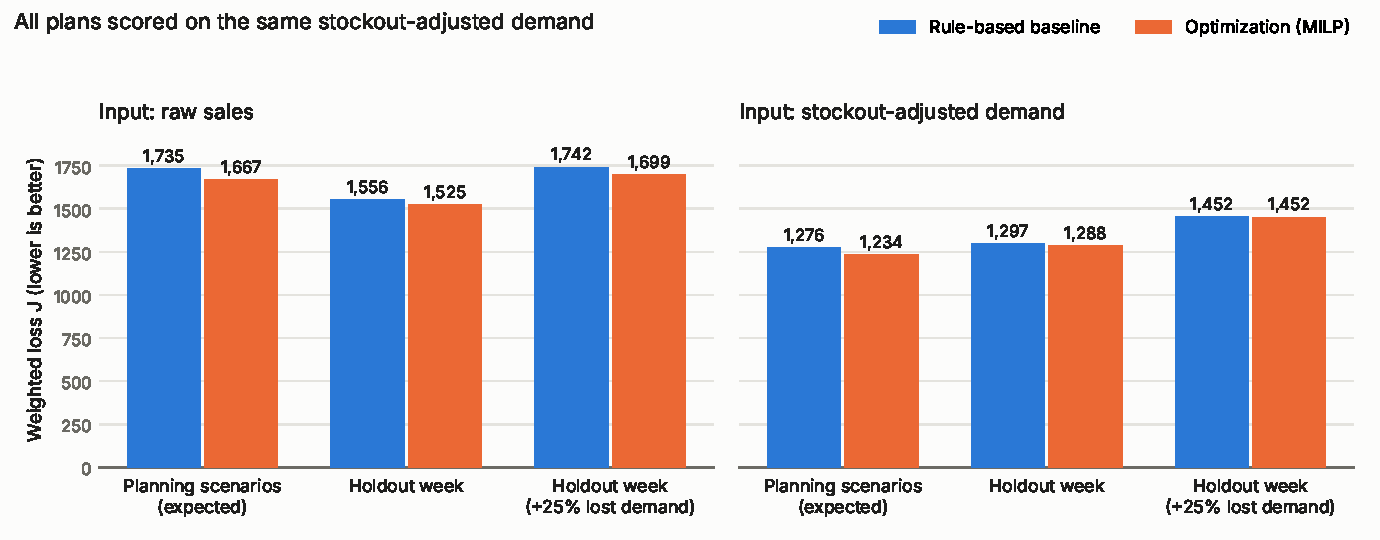
\includegraphics[width=.69\linewidth]{figures/fig_loss_2x2.pdf}
\caption{Four policies scored on the same evaluation demand, using base weights.}
\label{fig:loss2x2}
\end{figure}
The four-way MILP runs use HiGHS 1.16 with 900-second limits. Recovered-input and
raw-input gaps are 2.2\% and 11\%, respectively. The official M4 Gurobi plan is
shown separately. Solver precision qualifies small between-policy differences.

\clearpage
\section{Common-path performance and capacity diagnostic}
All policies are scored on corrected paths 11--2000, reserving paths 1--10 for
planning diagnostics. Mean fill rates below average path-level ratios.
Loss standard deviations measure variation across simulated weeks.
\begin{table}[H]\centering
\caption{Performance over 1,990 common MC paths. SD is the sample loss SD.}
\label{tab:mceval}
\begin{tabular}{llrrrr}\toprule
Input & Policy & Fill rate & Expired & Mean loss & Loss SD\\\midrule
Raw & Baseline & 71.7\% & 3.4 & 1,690.1 & 350.9\\
Raw & MILP & 72.2\% & 11.6 & 1,673.9 & 333.5\\
Recovered & Baseline & 78.4\% & 5.6 & 1,320.5 & 302.7\\
Recovered & MILP & 78.4\% & 12.5 & 1,331.8 & 290.5\\
Recovered & M4 Gurobi & 78.4\% & 15.0 & 1,330.9 & 288.5\\\bottomrule
\end{tabular}\end{table}
Recovery lowers mean loss by 21.9\% for baseline and 20.4\% for MILP, improving
both on every scoring path. Recovered MILP minus baseline loss averages
$+11.36$ (95\% paired CI $[10.49,12.24]$), or 0.86\% of baseline loss.
Baseline wins on 69.8\% of paths. For independent paths, the CI uses
$\bar\Delta\pm1.96s_\Delta/\sqrt{1990}$. It is conditional on the simulation model.
\begin{figure}[H]\centering
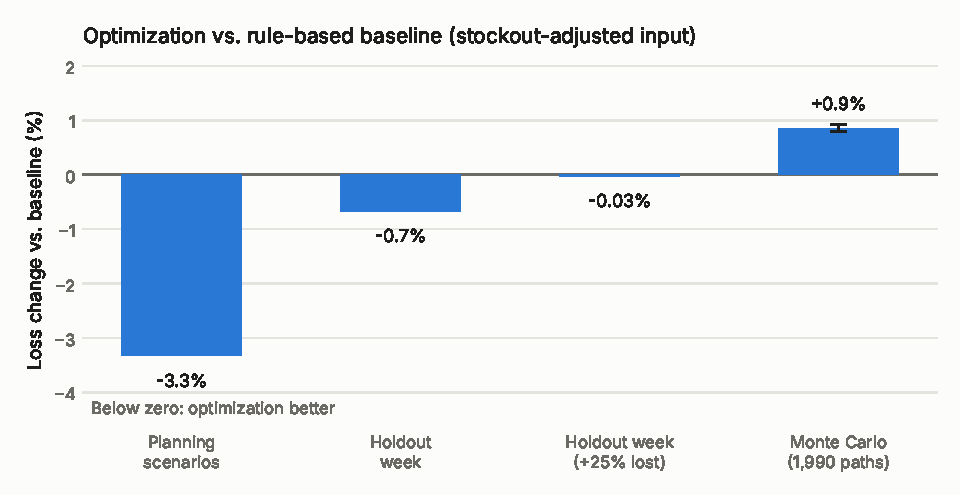
\includegraphics[width=.66\linewidth]{figures/fig_milp_vs_baseline.pdf}
\caption{Recovered-input MILP loss relative to baseline. The MC interval
measures paired simulation sampling error.}\label{fig:milpvsbase}
\end{figure}
Replanning on corrected quantile multipliers gives losses 1,342.5 (baseline)
and 1,353.7 (MILP), retaining a 0.83\% MILP disadvantage. Changing three
common multipliers alone leaves product-level inventory exposure unresolved.

\subsection{A feasibility--service trade-off}
Recovered baseline and MILP exceed storage at least once on every scoring path,
on 14.5 and 15.9 store-days on average. Requiring storage feasibility on ten
noisy planning paths gives a solver lower bound of 1,454.65 on those paths.
The original baseline scores 1,247.8 there while allowing overflow.
This demonstrates a cost of stricter scenario-wise feasibility relative to that
benchmark. The ten-path incumbent has a 13.7\% gap and orders about 818 units.
Its scoring loss is 1,795.6, 36\% above baseline. Its recorded metrics equal
the repaired-baseline start. Thus incumbent quality and feasibility restrictions
both matter when interpreting the diagnostic.

\clearpage
\section{Recommendations and limits}
\textbf{Prioritize demand correction.} Recovery has the largest measured effect
in this evaluation design. Monitor availability alongside sales and validate
recovery assumptions before setting replenishment targets.

\textbf{Pilot assortment and usable space.} Test 25 products per store, assess
incremental handling costs, and measure service and expiry. Storage expansion
merits assessment before extra supply at current settings. Protect current supply
reliability, since contraction materially reduces modeled service.

\textbf{Specify operational recourse before deployment.} The current MILP shows
limited out-of-sample benefit relative to the recovered baseline. Use this
baseline as a practical reference while defining how stores reject, discard, or
reschedule excess stock. A follow-up MILP can price these actions and allow
information-consistent adaptive deliveries. Apply identical operating rules when
comparing policies. Overflow costs and physical capacities must be measured.

\textbf{Limits.} Anonymous products, normalized resource use, assumed shelf life
and penalties, eight calibration weeks, one holdout week, and nonzero MIP gaps
qualify business interpretation. Evaluation demand shares recovery assumptions
with planning. Monte Carlo precision does not eliminate demand-model error.
Joint assortment--capacity investment effects remain to be tested.

\section{Code, data, and AI-use disclosure}
The public code and data repository is
\url{https://github.com/zhangjiayue-luna/ieor4004-group21l}.
The M5 files identify original planning data, corrected MC paths, saved policies,
sensitivity outputs, and v3 evaluation code. Gurobi requires a user-supplied license.
Reported plans and scoring inputs are retained for reproducing the tables.

\textbf{AI-use disclosure.} AI assisted reference search, code implementation,
visualization, numerical reconciliation, and report organization and wording.
Team members are responsible for understanding the submitted methods and code,
reviewing the assumptions, and the final interpretation.

\section*{References}
Chen, L.-M., \& Sapra, A. (2013). Joint inventory and pricing decisions for
perishable products with two-period lifetime. \textit{Naval Research Logistics,
60}(5), 343--366. \url{https://doi.org/10.1002/nav.21538}

Dingdong-Inc. (2025). \textit{FreshRetailNet-50K} [Data set]. Hugging Face.
\url{https://huggingface.co/datasets/Dingdong-Inc/FreshRetailNet-50K}

Gurobi Optimization. (n.d.). \textit{Python API reference}.
\url{https://docs.gurobi.com/projects/optimizer/en/current/reference/python/model.html}

Shi, C., Chen, W., \& Duenyas, I. (2016). Technical note---Nonparametric data-driven
algorithms for multiproduct inventory systems with censored demand.
\textit{Operations Research, 64}(2), 362--370.
\url{https://doi.org/10.1287/opre.2015.1474}
\end{document}
